\begin{frame}{Introduction to Transformers}
  \begin{itemize}
    \item[$\blacktriangleright$] \textbf{What is a Transformer?}
    \begin{itemize}
      \item Introduced by Vaswani et al.\ (2017) -- ``Attention is All You Need''
    \end{itemize}
    \vspace{0.6em}
    \item[$\blacktriangleright$] \textbf{Key features:}
    \begin{itemize}
      \item No recurrence, all attention
      \item Encoder-decoder structure
      \item Enables parallel processing
      \item Scales well with data and compute
    \end{itemize}
  \end{itemize}
\end{frame}

\begin{frame}{Transformer Architecture: Components Overview}
  \begin{columns}
    \begin{column}{0.53\textwidth}
      \begin{itemize}
        \item[$\blacktriangleright$] Tokenization
        \item[$\blacktriangleright$] Input Embeddings
        \item[$\blacktriangleright$] Position Encodings
        \item[$\blacktriangleright$] Query, Key, \& Value
        \item[$\blacktriangleright$] Attention
        \item[$\blacktriangleright$] Self Attention
        \item[$\blacktriangleright$] Multi-Head Attention
        \item[$\blacktriangleright$] Feed Forward
        \item[$\blacktriangleright$] Add \& Norm
        \item[$\blacktriangleright$] Encoders
        \item[$\blacktriangleright$] Masked Attention
        \item[$\blacktriangleright$] Encoder Decoder Attention
        \item[$\blacktriangleright$] Linear
        \item[$\blacktriangleright$] Softmax
        \item[$\blacktriangleright$] Decoders
        \item[$\blacktriangleright$] Encoder-Decoder Models
      \end{itemize}
    \end{column}
    \begin{column}{0.47\textwidth}
      \centering
      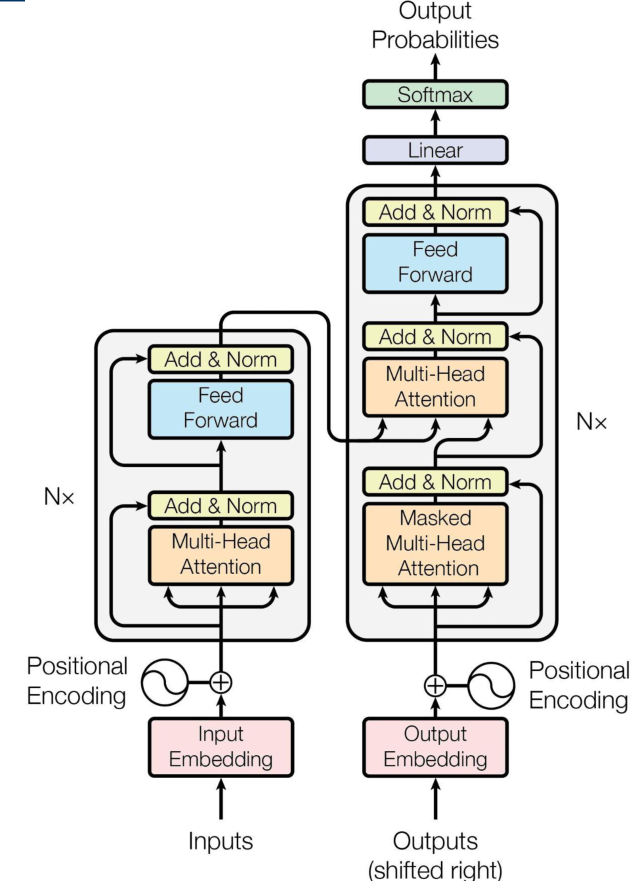
\includegraphics[width=0.9\linewidth,height=0.78\textheight,keepaspectratio]{images/introduction-to-transformers/transformer_vaswani_encoder_decoder_diagram.png}

      {\scriptsize Source: Vaswani et al., ``Attention Is All You Need,'' NeurIPS 2017, Fig.~1.}
    \end{column}
  \end{columns}
\end{frame}

\begin{frame}{Machine Translation}
  \centering
  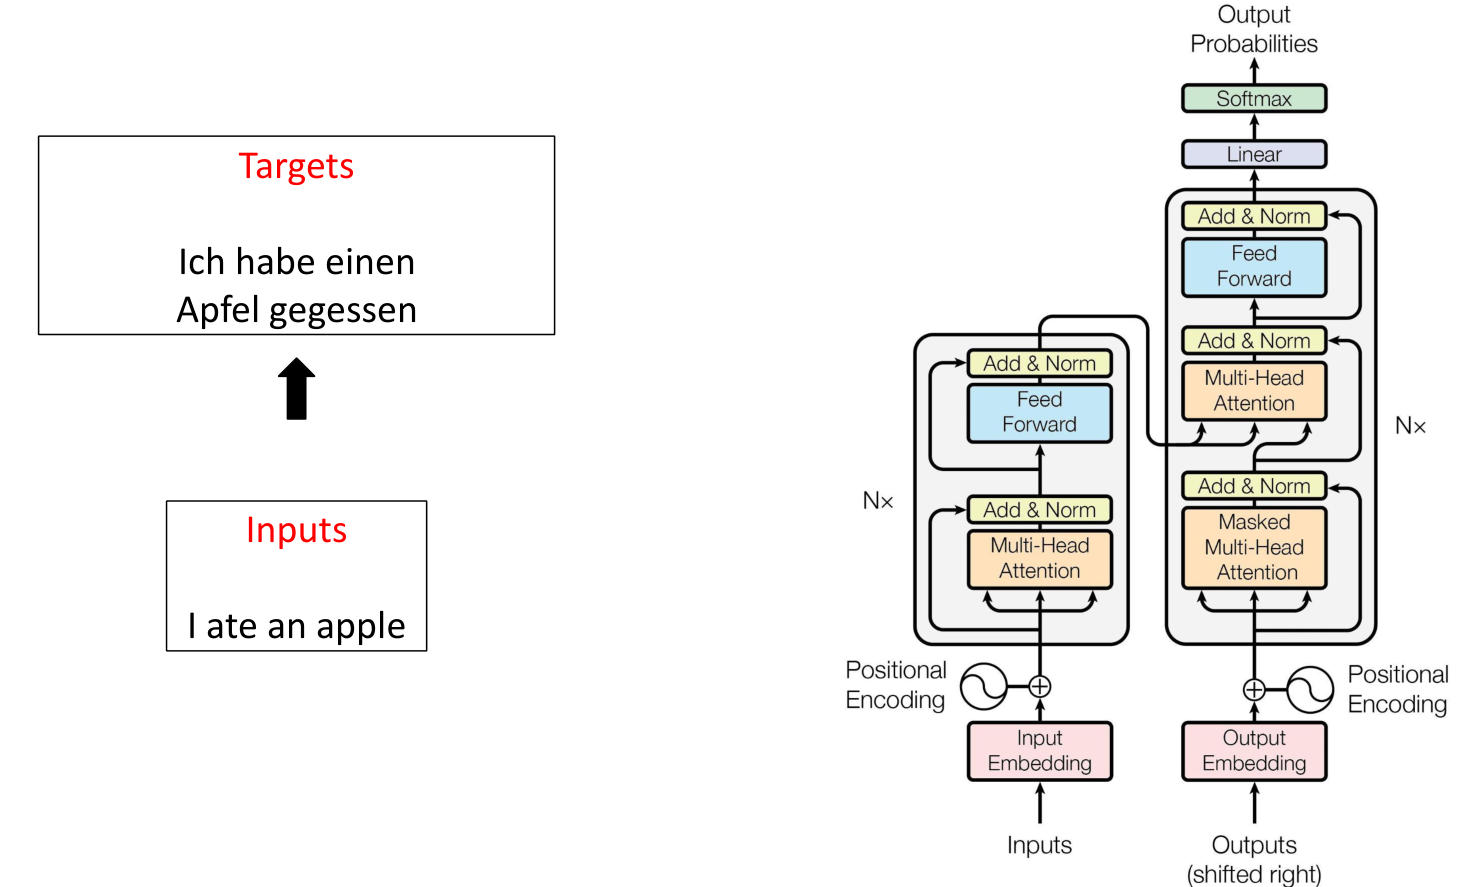
\includegraphics[width=0.8\paperwidth,height=0.75\paperheight,keepaspectratio]{images/introduction-to-transformers/transformer_translation_inputs_targets_example.png}

  {\scriptsize Source: CMU 11-785, Lecture 19 ``Transformers,'' Spring 2024, slide 7.}
\end{frame}

\begin{frame}{Inputs}
  \centering
  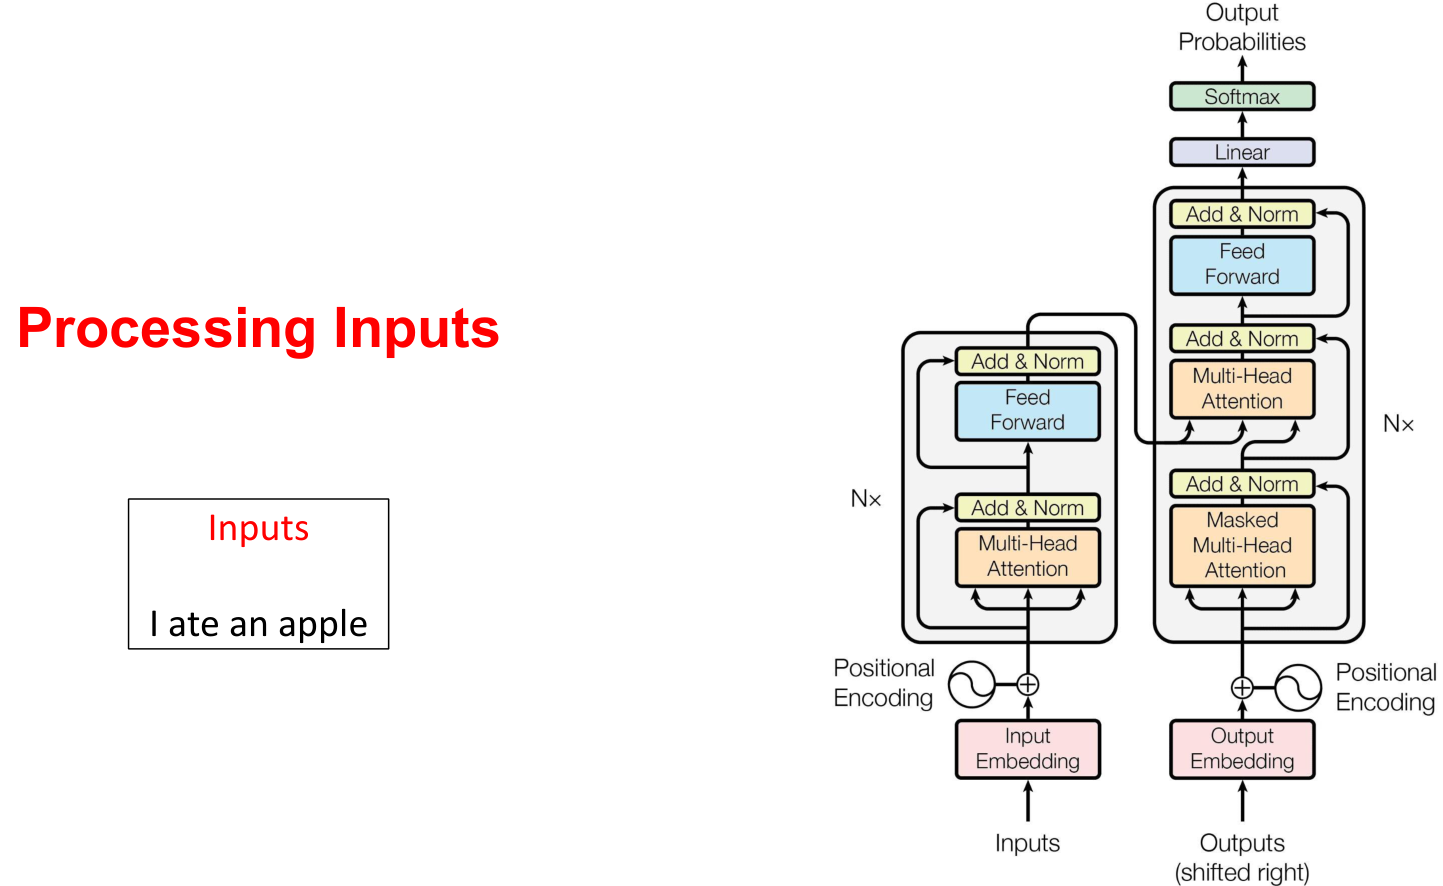
\includegraphics[width=0.8\paperwidth,height=0.75\paperheight,keepaspectratio]{images/introduction-to-transformers/transformer_processing_inputs_example.png}

  {\scriptsize Source: CMU 11-785, Lecture 19 ``Transformers,'' Spring 2024, slide 8.}
\end{frame}
